%!TEX root = ../main.tex
%\documentclass{standalone}
%\begin{document}

We implement the algorithms in Section~\ref{sec:algorithm} on top of OSTRICH~\cite{Ostrich,atva2020}, resulting in a version of OSTRICH called $\ostrichrecl$.
Then we do experiments on two benchmark suites to evaluate the performance of $\ostrichrecl$, and carry out detailed experiments, including the evaluation of size-reduction techniques and the experiment of large-counting benchmark. In the sequel, we first describe the two benchmark suites, then present the settings and results of the experiments.

%This section presents the empirical evaluation of OstrichCEA, which is our implementation of the decision procedure introduced in Section \ref{sec:algorithm}. Our objective is to validate the effectiveness of the proposed techniques by evaluating our tool's correctness and efficiency compared to other solvers. Furthermore, we assess the efficacy of our heuristics by testing different configurations of the tool. We have implemented our encoding for counting with two heuristic algorithms on Ostrich+ \cite{atva2020}. The pre-image computation for concatenation, \verb|indexOf|, \verb|substring|, \verb|replaceAll|, \verb|reverse| and finite transducer remain unchanged. OstrichCEA is written in Scala and based on the SMT solver Princess\cite{princess}.

\vspace{-3mm}
\subsection{Benchmark Suites and Experiment Setup}\label{sec:bench}
\vspace{-2mm}

Our experiments utilize two benchmark suites, namely, RegCoL and AutomatArk. In total, there are 48,843 instances in the two benchmark suites. All the benchmark instances are in SMTLIB2 format.

\medskip
\noindent
\emph{RegCoL benchmark suite.} There are 40,628 RECL constraints in the RegCoL suite. These constraints are generated by extracting regular expressions with counting operators from the open source regex library \cite{regex_lingua_franca,redos_lenka} and constructing for each regular expression $e$ a RECL constraint of the form
$x \in e \wedge x \in \overline{\Sigma^*(<+ >+'+''+\&)\Sigma^*} \wedge |x| > 10,$
where $\overline{\Sigma^*(<+ >+'+''+\&)\Sigma^*}$ is a regular expression that sanitizes all occurrence of special characters $<$, $>$, $'$, $''$, or $\&$. The artificial construction is meaningful because the special characters are offensive. For instance, they are widely used in client-side attacks like XSS\cite{malware_detection_3_kudzu,CCH_18}.
%We would like to remark that there are about 500,000 real-world regular expressions in \cite{regex_lingua_franca,redos_lenka} and regular expressions with counting operators occupy about 8\% of them. 

\medskip
\noindent
\emph{AutomatArk benchmark suite.}
The AutomatArk benchmark suite is adapted from the AutomatArk suite in \cite{z3str3re} by filtering out the string constraints that contain no occurrences of counting operators and adding the length constraint $|x| > 10$ (where $x$ is a string variable). There are 8,215 instances in the AutomatArk suite here.
Note that the original AutomatArk benchmark suite in \cite{z3str3re} includes 19,979 instances, conjunctions of regular membership queries generated out of regular expressions from \cite{automatark}.
%Only 8,751 contain counting operators out of 19,979 instances. 
Moreover, only 5\% of them include non-register-representable regexes among the 48,843 instances.
%%%%%%%%%%%%%%%%%% the benchmark suite written by Denghang %%%%%%%%%%%
%%%%%%%%%%%%%%%%%% the benchmark suite written by Denghang %%%%%%%%%%%

\medskip
\noindent
\emph{Experiment setup.}
All experiments are conducted on CentOS Stream release 8 with 4 Intel(R) Xeon(R) Platinum 8269CY 3.10GHz CPU cores and 190 GB memory. We use the \textsc{zaligvinder} framework \cite{zaligvinder_2021} to execute the experiments, with a timeout of 60s for each instance.
\hide{
  We conducted a comparison on four sets of benchmarks based on regex with
  counting operator, consisting of a total of 49,379 instances. We analyze all 19 developed benchmarks listed in \cite{zaligvinder_2021} and find that only \textbf{AutomatArk} benchmarks have regular membership with the counting operator. In total, almost 18\% of the instances we evaluated were sourced from published industrial benchmarks or other solver developers. The other instances are generated by ourselves with regular expressions from the real world. Each set of the benchmark is evenly divided into "large" and "small": the "large" set contains instances with large upper bounds of the counting operator (the sum of upper bounds is greater than 50), and "small" contains remaining instances. About 10\% of the benchmarks are in a "large" set. More details about the benchmarks are shown below.

  \subsubsection{AutomatArk} is the 8,751 instances generated by Berzish et al.\cite{z3str3re}. It is based on real-world regular expression queries from Loris D'Antoni\cite{automatark}. The origin set comprises two tracks, a simple and a hard track, with 19,979 instances. The simple track contains instances with a single regular expression membership constraint, whereas the hard track can hold up to five membership constraints for a single variable per instance. We extract 8,751 instances containing counting operators.

  \subsubsection{ReDos} is the set of 1,624 instances we generated. It is based on the ReDos-attacked regular expression collected by Lenka et al. For each regular expression, we generate an instance as the template (\ref{eq:template}) where $\regex$ is the regular expression. The regular membership predicate $x\not\in \Sigma^*(<\mid >\mid '\mid ''\mid \&)\Sigma^*$ sanitizes the input string $x$ to avoid the attack. The length lower bound is set to $20$ for the "small" set and $50$ for the "large" set.

  \subsubsection{RegexLib} is the set of 1,623 instances we generated similarly to the \textbf{ReDos} benchmark. It is based on the regular expressions collected by James C. Davis et al.\cite{regex_lingua_franca} from regex lib website\cite{regexlib}. The website is the Internet's first Regular Expression Library. Currently, it has indexed 4149 expressions from 2818 contributors around the world since 2001. We extracted 1,623 instances containing bounded repetition from 4149 instances. The length lower bound is set to $20$ for the "small" set and $50$ for the "large" set.

  \subsubsection{StackOverflow} is the 37381 instances we generated similarly to the \textbf{ReDos} benchmark. As the Regexlib benchmark, the real-world regex expressions are collected by James C. Davis et al.\cite{regex_lingua_franca} from StackOverflow website\cite{stackoverflow}. The website is a question-and-answer site for professional and enthusiast programmers. We extracted 37,381 instances containing bounded repetition from almost 500,000 instances. The length lower bound is set to $20$ for the "small" set and $50$ for the "large" set.
  \begin{equation} \label{eq:template}
    x\in \regex \wedge x\not\in \Sigma^*(<\mid >\mid '\mid ''\mid \&)\Sigma^*\wedge |x| > 50(or \ 20)
  \end{equation}
}
%%%%%%%%%%%%%%%%%% the benchmark suite written by Denghang %%%%%%%%%%%
%%%%%%%%%%%%%%%%%% the benchmark suite written by Denghang %%%%%%%%%%%

\vspace{-3mm}
\subsection{Overall Experiment Results}
\vspace{-2mm}

We evaluate the performance of $\ostrichrecl$ against the state-of-the-art string constraint solvers, including CVC5
%(version 1.0.5) 
\cite{cvc5}, Z3seq \cite{z3seq}, Z3str3
%(github commit 59e9c87) 
\cite{z3str3}, Z3str3RE \cite{z3str3re}, and OSTRICH
%(github commit 8297d8d) 
\cite{ostrich2023}, on RegCoL and AutomatArk benchmark suites.
% Z3-trau \cite{z3trau} is not evaluated because it does not support \verb|re.diff|, the language difference operator of regular expressions.  
%The experiments are designed to answer the following two research questions. 
%\begin{description}
%\item[Q1] Does OSTRICH$^{\rm RECL}$ solve RECL constraints more efficiently than the state-of-the-art string constraint solvers ?
%
%\item[Q2] Do the size-reduction and under-approximation techniques proposed in Section~\ref{sec:algorithm} indeed improve the performance ?
%\end{description}
\vspace{-5mm}
\begin{table}
  \centering
  \begin{subtable}{0.513\textwidth}
      \centering
      \import{tables}{table_regcol.tex}
      \caption{Overall experiment results,\\ with timeout = 60 seconds.}
      \label{tab:results_regcol}
  \end{subtable}
  \begin{subtable}{0.477\textwidth}
      \centering
      \import{tables}{table_simp.tex}
      \caption{Simplification technique evaluation, with timeout = 60 seconds.}
      \label{tab:results_simp}
  \end{subtable}
  \vspace{-6mm}
  \caption{Experiments on RegCoL and AutomatArk benchmark suites}
\end{table}
\vspace{-9mm}
% \begin{table}[ht]
%   \vspace{-5mm}
%   \begin{center}
%     \import{tables}{table_regcol.tex}
%   \end{center}
%   \caption{Overall Experiment results, with timeout = 60 seconds}
%   \label{tab:results_regcol}
%   \vspace{-9mm}
% \end{table}

The overall experiment results are in Table~\ref{tab:results_regcol}. Note that we take the result of CVC5 as the ground truth\footnote{At first we used the majority vote between all results of the solvers as the ground truth, but solvers of z3 family output some wrong results(verified by us manually), causing the ground truth to be incorrect.}. We can see that $\ostrichrecl$ solves almost all 48,843 instances, except 182 of them, that is, it solves \textbf{48,662} instances correctly. The number is %3,994/2,272/24,577/12,832/1,091/7,092 
\textbf{3,908/1,111/12,838/2,306/2,396 more} than the number of instances solved by CVC5/Z3str3RE/Z3str3/Z3seq/OSTRICH respectively.
%      
%A soundness error is reported if the result of a solver for an instance is different from CVC5. 
% their results on some instances are inconsistent with the results of the other three solvers, i.e. CVC5, OSTRICH, and OSTRICH$^{\rm RECL}$.
%
Moreover, our solver $\ostrichrecl$ is the second fastest solver, and its average time on each instance is close to the fastest solver Z3str3RE (\textbf{1.93}/1.62 s).
\vspace{-3mm}
\subsection{Evaluation of Simplification Techniques}
\vspace{-2mm}

We evaluate the simplification techniques by comparing the performance of $\ostrichrecl$ with and without the simplification techniques. Moreover, we also encode the $\cefadec$ problem to an infinite state transition system and solve it using \textsc{nuXmv}\cite{nuxmv}. 
% \begin{table}[ht]
%   \vspace{-5mm}
%   \begin{center}
%     \import{tables}{table_simp.tex}
%   \end{center}
%   \caption{Simplification technique evaluation, with timeout = 60 seconds}
%   \label{tab:results_simp}
%   \vspace{-9mm}
% \end{table}

The evaluation results of simplification techniques are in Table~\ref*{tab:results_simp}. Compared to $\ostrichrecl$ without simplification techniques, $\ostrichrecl$ with simplification techniques solves \textbf{1,503 more} instances and is \textbf{2.21$\times$} faster. Moreover, compared with the techniques using \textsc{nuxmv}, $\ostrichrecl$ with simplification techniques solves \textbf{1,798 more} instances and is \textbf{3.13$\times$} faster. 

\vspace{-3mm}
\subsection{Large-Counting Experiment Results}
The distribution of upper bounds of counting in RegCoL and AutomatArk suites is shown in Fig~\ref{fig:count_distri}, whose horizontal axis is the value of the upper bound and vertical axis is the number of occurrences. The upper bound is the number $n$ of regex $e^{\{m,n\}}, e^{\{n,n\}}$ and $e^{\{n,\infty\}}$ (which is equivalent to $e^{\{n,n\}}e^*$). Although most upper bounds of counting operators are less than 50, about two thousand are still greater than 50. We extract instances with upper bounds greater than 50 and generate a \emph{`large-counting'} benchmark suite (1,969 instances in total). Moreover, We change the length constraint of each instance to $|x| > 200$ (which is $|x| > 10$ in the overall experiment), to make the suite more balanced.
\vspace{-5mm}
\begin{figure}[ht]
  \centering
  \begin{subfigure}[t]{0.49\textwidth}
    \centering\vskip 0pt
    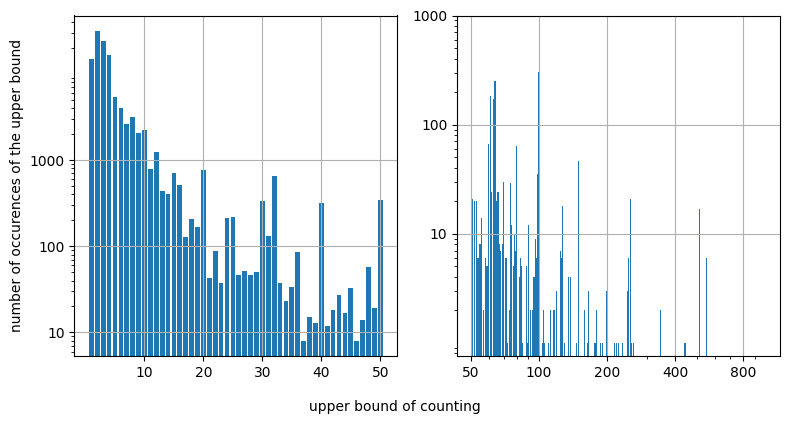
\includegraphics[width=1\textwidth]{counting_distribution.png}  
    \caption{Distribution of counting operators in two benchmark suites.}  
    \label{fig:count_distri}
  \end{subfigure}
  \hfill
  \begin{subfigure}[t]{0.49\textwidth}
    \centering\vskip 0pt
    \import{tables}{table_large_count.tex}
    \vspace{4.5mm}
    \caption{Large-counting experiment, \\with timeout = 60 seconds.}
    \label{fig:table_large_count}
  \end{subfigure}
  \vspace{-2mm}
  \caption{Analysis of dataset and large-counting experiment.}
\end{figure}
\vspace{-5mm}

% \begin{table}[ht]
%   \vspace{-5mm}
%   \begin{center}
%     \import{tables}{table_large_count.tex}
%   \end{center}
%   \caption{Large-counting experiment, with timeout = 60 seconds}
%   \label{tab:results_simp}
%   \vspace{-9mm}
% \end{table}

We evaluate the performance of $\ostrichrecl$ on these instances. The results are in Fig~\ref{fig:table_large_count}. We can see that $\ostrichrecl$ solves \textbf{1,873} instances correctly, which is \textbf{947/278/563/637/523 more} than the number of instances solved by CVC5/Z3str3RE/Z3str3/Z3seq/OSTRICH respectively. Moreover, \newline
$\ostrichrecl$ is the fastest solver, who is \textbf{ 6.79/2.88/2.61/5.27/3.95$\times$ } faster than CVC5/Z3str3RE/Z3str3/Z3seq/OSTRICH respectively.
\vspace{-2mm}



% The results are in Table~\ref{tab:results_simplification}. We can see that the simplification technique improves the performance of $\ostrichrecl$ significantly. It solves 1,111 more instances and is 1.62 times faster than $\ostrichrecl$ without the simplification technique.

% \begin{table}[ht]
% %\vspace{-1mm}
% \begin{center}
%   \import{tables}{table_automatark.tex}
% \end{center}
%   \caption{Experiment results on AutomatArk, with timeout = 60 seconds}
%   \label{tab:results_automatark}
% \vspace{-6mm}
% \end{table}

% The experiment results on the AutomatArk benchmark suite are put in Table~\ref{tab:results_automatark}. 
% From Table~\ref{tab:results_automatark}, we can see that $\ostrichrecl$ solvers almost all 8,215 instances, except 39 of them, that is, it solves 8,176 instances correctly, which is %3,994/2,272/24,577/12,832/1,091/7,092 
% 101/191/4,094/2,632/9/1,587
% more than the number of instances solved by CVC5/Z3seq/Z3-Trau/Z3str3/Z3str3RE/OSTRICH respectively. 
% %    
% Still, the soundness errors are reported by taking the results of CVC5 as the ground truth.
%Note that Z3-Trau has soundness errors, where the result of CVC5 is taken as the ground truth. If CVC5 reports ``unknown'' or ``timeout'' in some instances, then no soundness errors will be reported in this instance. 
%A soundness error is reported if the result of a solver for an instance is different from CVC5. 
% their results on some instances are inconsistent with the results of the other three solvers, i.e. CVC5, OSTRICH, and OSTRICH$^{\rm RECL}$.
%
% Moreover, $\ostrichrecl$ spends 2.49 seconds per instance on average. 
%while the fastest solver Z3str3RE spends 1.71 seconds per instance, and the other solvers spend at least 3.49 seconds per instance.  
%Note that Z3-Trau reports ``unknown'' on 2,552 instances, which seems to be mainly attributed to the fact that it does not support \verb|re.diff|, the language difference operator of regular expressions. 

% In summary, $\ostrichrecl$ solves 48,698 out of 48,843 instances, 1,091 more than Z3str3RE, the state-of-the-art best solver on RECL constraints. Moreover, the speed of $\ostrichrecl$ is the second fastest and comparable to that of Z3str3RE. (See Table~\ref{tab:results_summary}.)

% \begin{table}[ht]
% \vspace{-3mm}
% \begin{center}
%   \import{tables}{table_summary.tex}
% \end{center}
%   \caption{Experiment results: A Summary}
%   \label{tab:results_summary}
% \vspace{-6mm}
% \end{table}


%Q1 is answered by running OSTRICH$^{\rm RECL}$ and the aforementioned solvers on AutomatArk and RegCoL. 

%\zhilin{may add the results for the two benchmark suites separately.}


%%%%%%%%%%%%%%%%%% Q2 removed %%%%%%%%%%%%
%%%%%%%%%%%%%%%%%% Q2 removed %%%%%%%%%%%%
\hide{
  \begin{table}[ht]
    \vspace{-3mm}
    \begin{center}
      \subimport{tables}{table_heuristic.tex}
    \end{center}
    \caption{Experiment results for Q2, where the timeout period is 60 seconds}
    \label{tab:results_heuristics}
    \vspace{-6mm}
  \end{table}

  To answer Q2, we compare OSTRICH$^{\rm RECL}$ with its three variants, namely, OSTRICH$^{\rm RECL}$ where the size-reduction, under-approximation, or both are removed.
  For convenience, let us use OSTRICH$^{\rm RECL^-}$ to denote the variant of OSTRICH$^{\rm RECL}$ that both size-reduction and under-approximation techniques are removed,
  OSTRICH$^{\rm RECL^-}_{+\rm SR}$ (resp. OSTRICH$^{\rm RECL^-}_{+\rm UA}$) to denote the variant that is obtained by adding the size-reduction (resp. under-approximation) techniques to OSTRICH$^{\rm RECL^-}$.
  %OSTRICH$^{\rm RECL}_{\rm -SR}$, OSTRICH$^{\rm RECL}_{\rm -UA}$, OSTRICH$^{\rm RECL}_{\rm -SRUA}$, which remove size-reduction, under-approximation, and both from OSTRICH$^{\rm RECL}$ respectively. 
  The experiment results can be found in Table~\ref{tab:results_heuristics}.
  From Table~\ref{tab:results_heuristics}, we can see that adding size-reduction techniques help to solve 1,563 more instances and reduce the average time per instance for 46.4\% (see the OSTRICH$^{\rm RECL^-}_{\rm +SR}$ column), while adding under-approximation techniques help to solve 1,476 more instances and reduce the average time per instance for 42.7\% (see the OSTRICH$^{\rm RECL^-}_{\rm +UA}$ column), moreover, adding both help to solve 1,579 more instances and reduce the average time per instance for 46.5\% (see the OSTRICH$^{\rm RECL}$ column). Note that adding under-approximation to OSTRICH$^{\rm RECL^-}_{\rm +SR}$ helps to solve 19 more sat instances while reducing the number of solved unsat instances by 3 since under approximation techniques do not help to solve unsat instances.
}
%%%%%%%%%%%%%%%%%% Q2 removed %%%%%%%%%%%%
%%%%%%%%%%%%%%%%%% Q2 removed %%%%%%%%%%%%
%Moreover, adding these techniques also decrease the average time spent in solving each instance considerably.


%\zhilin{stopped here}

%%%%%%%%%% original texts by denghang %%%%%%%%%
%%%%%%%%%% original texts by denghang %%%%%%%%%
\hide{
  %
  We have evaluated OstrichCEA compared to five other prominent string solvers currently available. We evaluate the solvers by directly comparing the number of cases correctly solved, the average time taken with and without timeouts, and the total count of soundness errors and program crashes. One of these solvers is CVC5\cite{cvc5}, a general SMT solver that uses algebraic reasoning to handle strings and regular expressions and is the winner of SMT-COMP 2022\cite{smt-comp}. Another solver, Z3str3\cite{z3str3}, is the most recent edition we can get to the Z3-str family and utilizes a word equation reduction approach to reason about regular expressions. Z3str3RE\cite{z3str3re} is a variant of Z3str3 that incorporates length-aware algorithms and heuristics. Z3seq\cite{z3seq} is a sequence solver which uses a novel derivative theory for solving extended regular expressions. Z3-Trau\cite{z3trau} is the Z3 version of trau\cite{trau} that employs a flat automata-based approach, incorporating both under- and over-approximations. Ostrich\cite{Ostrich} is the tool we extend which uses automaton to model the semantics of string functions and regular memberships. We used the 1.0.5 binary version of CVC5, commit 59e9c87 of Z3str3, the last version of Z3str3RE, 4.8.9 binary version of Z3Seq, commit 1628747 of Z3-Trau and commit 8297d8d of Ostrich. Z3-Trau does not support \verb|re.diff|. All other solvers support all syntax sugars listed in SMT-LIB standard\cite{smt_lib}. We omitted Z3str4\cite{z3str4} because the provided reproduction package link is wrong. All experiments are conducted on CentOS Stream release 8 with 12 Intel(R) Xeon(R) Platinum 8269CY CPU T 3.10GHz processors and 190 GB memory. We used Zaligvinder\cite{zaligvinder_2021} framework and set the timeout to 60 seconds.

  %\subsection{Overall Evaluation}
  In Fig.\ref{fig:cactus_all}, the cactus plot illustrates the cumulative time each solver takes for all cases in ascending order of runtime. Solvers located towards the right and lower portion of the plot indicate better performance. \newline
  Table \ref{tab:results_all} summarizes the results demonstrating OstrichCEA's superior performance, solving the most significant number of instances and outperforming most competing solvers. Including timeouts, OstrichCEA is \textbf{1.52}\mult{} faster than Z3Seq, \textbf{2.23}\mult{} faster than Ostrich, \textbf{2.26}\mult{} faster than Z3-Trau, \textbf{3.08}\mult{} faster than Z3str3, \textbf{3.11}\mult{} faster than CVC5 and close to Z3str3RE with \%2 speed loss . Note that CVC5\cite{cvc5} yielded 5370 timeouts(11\% of all instances), and Z3str3\cite{z3str3} yielded 6139 timeouts(12\% of all instances), which is much more than other solvers. Both CVC5 and Z3str3 are DPLL(T)-based solvers. It seems that almost 10\% of the benchmarks we used seem unsuitable for them. Z3-trau\cite{z3trau} yielded 21,152 unknowns because it does not support \verb|re.diff|. Z3-trau\cite{z3trau} yielded 6673 crashes (13\% of the instances) and 1233 soundness errors (2\% of the instances), which is a large portion. Z3-based solvers Z3str3 yielded 38 soundness errors, Z3seq\cite{z3seq} yielded 51 soundness errors and Z3str3RE\cite{z3str3re} yielded 39 soundness error. Most of them are due to the mistake of formalization of the backslash character. OstrichCEA resulted in 5 unknowns because it reached the maximum threshold of limited memory 2GB. More details of the results of each benchmark are shown in \ref{appendix:experiential_results}.
  \begin{figure}[h]
    \centering
    \import{figures}{cactus_plot_all.tex}
    \caption{Cactus plot summarizing performance on all benchmarks.}
    \label{fig:cactus_all}
  \end{figure}

  %\subsection{Analysis of Individual Heuristics}
  In order to demonstrate the efficacy of the individual heuristics outlined in Section \ref{sec:algorithm} and incorporated into OstrichCEA, we assessed various tool configurations in which one or more heuristics were disabled. Figure \ref{fig:cactus_heuristics} and Table \ref{tab:results_heuristics} display the outcomes. The "OstrichCEA" plot line represents the tool's performance when all heuristics are enabled, while the "All heuristics off" line represents performance when all heuristics are disabled. The remaining plot lines exhibit performance with only the named heuristic disabled while all others are enabled. The plots and table show that OstrichCEA functions most effectively when all heuristics are enabled. In average time with timeout times, OstrichCEA performs \textbf{1.78}$\times$ faster than employing none of our heuristics, \textbf{1.37}$\times$ faster than turning off simplification, \textbf{1.15}$\times$ faster than truing off under-approximation.
  \begin{figure}
    \subimport{figures/}{cactus_plot_heuristic.tex}
    \caption{A performance comparison was made on all benchmarks by turning off individual heuristics using a cactus plot.}
    \label{fig:cactus_heuristics}
  \end{figure}
  \begin{table}
    \subimport{tables}{table_heuristic.tex}
    \caption{A performance comparison was made on all benchmarks by turning off individual heuristics.}
    \label{tab:results_heuristics}
  \end{table}
}
%%%%%%%%%% original texts by denghang %%%%%%%%%
%%%%%%%%%% original texts by denghang %%%%%%%%%
%\end{document}